\section{ZigBee}

ZigBee jest standardem transmisji bezprzewodowej zapewniający niskokosztową platformą
możliwą do zastosowania w elektronice użytkowej, automatyce domowej, wszelkiego rodzaju sensorach
(w~szczególności przemysłowych i~medycznych) jak również grach i~zabawkach.
Pierwsza specyfikacja opublikowana została w grudniu 2004 roku będąc ciągle aktualizowana,
z najnowszą jej wersją będącą datowaną na marzec 2017 roku~\cite{zigbee_alliance_zigbee_2017}.

Architektura ZigBee oparta została o IEEE 802.15.4. Definiuje ona fundamentalne zagadnienia:
\gls{PHY} i~\gls{MAC}. Warstwa fizyczna odpowiada za funkcjonowanie
radia, \gls{LQI}, transmisję danych i~odbiór pakietów poprzez łącze fizyczne. Definiuje dozwolone
częstotliwości działania, szerokości pasma, rodzaj modulacji i~dozwoloną przepustowość danych
wyrażonych w bitach na sekundę. Warstwa MAC odpowiada za komunikację w wyższych warstwach stosu.
Obejmuje to między innymi zarządzanie dostępem do kanałów, walidacja ramek danych, informację
zwrotną o~otrzymaniu i~przetworzeniu danych~\gls{ACK} oraz zapewnia odpowiednie
uchwyty celem umożliwienia wdrożenia mechanizmów zabezpieczeń.
Standard wprowadza również pojęcie topologii uwzględniając tym samym sposoby,
w~jakich można zorganizować sieć poszczególnych urządzeń. Definiowane są dwie
opcje połączeń: gwiazda, peer-to-peer. Topologia gwiazdy pozwala podłączenie wielu węzłów
uwzględniając fakt, iż komunikacja odbywa się za pośrednictwem koordynatora \gls{PAN},
będący tożsamy z \gls{FFD}. W~przypadku konfiguracji rówieśniczej, urządzenia mogą 
komunikować się dodatkowo między sobą, zapewniając możliwość ustanowienia innych struktur, m.in. 
Mesh. Standard wprowadza określenie \gls{RFD}, będące najczęściej urządzeniem o~prostej funkcjonalności 
niewymagającym dużych ilości danych do funkcjonowania, o~zredukowanej potrzebie na 
zasoby sprzętowe~\cite{ieee_p80215_working_group_ieee_nodate}.

\begin{figure}[!ht]
	\centering 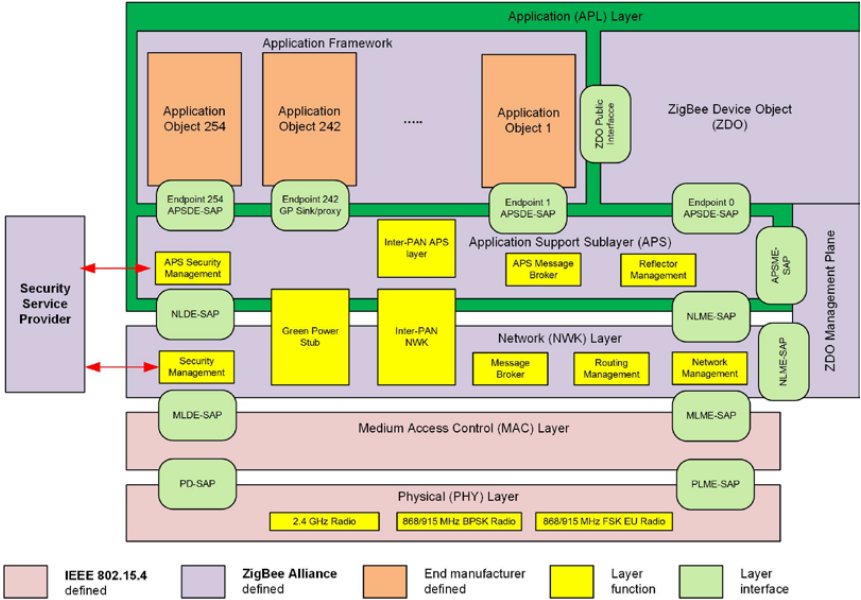
\includegraphics[width=0.99\linewidth]{zigbee_stack_architecture.png}
	\caption{Architektura stosu ZigBee. Źródło:~\cite{zigbee_alliance_zigbee_2017}}
	\label{rys:zigbee_stack_architecture}
\end{figure}

Specyfikacja ZigBee, opierając się na dokumentach IEEE 802.15.4, wykorzystuje częstotliwości
$868/915 MHz$ (w zależności od regionu Europa albo USA/Australia) oraz 2.4GHz~\cite{zigbee_alliance_zigbee_2017}.
Umożliwia tym samym transfer z przepustowością do 250~kbps~\cite{silicon_laboratories_ug10302_2021}.
Omawiany standard wprowadza swoje dodatkowe warstwy komunikacji do stosu: \gls{NWK} oraz~\gls{APL} --
Rysunek~\ref{rys:zigbee_stack_architecture}.
Warstwa aplikacji, będącą najwyższą w~hierarchi, składa się z wielu składowych. \gls{APS} odpowiada za
komunikację pomiędzy \gls{NWK} a~warstwami wyższymi. Oferuje między innymi parowanie urządzeń,
przekazywanie wiadomości, adresację, zajmuje się fragmentacją pakietów i~zapewnia niezawodny transport danych.
\gls{ZDO} w~głównej mierze odpowiada za wyszukiwanie urządzenia i~usług ZigBee~\cite{stmicroelectronics_an5506_2020, zigbee_alliance_zigbee_2017}.
Nadaje on również role urządzeniom sieci.

\begin{figure}[!ht]
	\centering 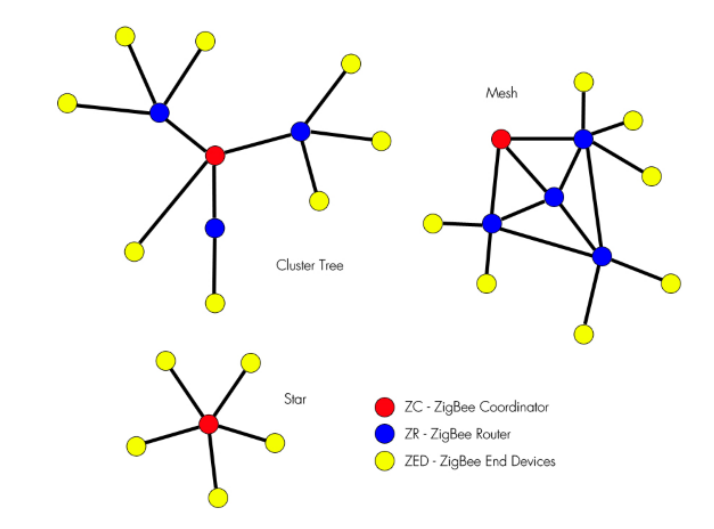
\includegraphics[width=0.618\linewidth]{zigbee_topologies_an5506.png}
	\caption{Topologie sieci ZigBee. Źródło:~\cite{stmicroelectronics_an5506_2020}}
	\label{rys:zigbee_topologies_an5506}
\end{figure}

ZigBee wprowadza trzy główne definicje ról urządzeń rejestrowanych do wewnątrz sieci:
\begin{itemize}
\item \gls{ZC} -- węzeł odpowiadający za utworzenie i~utrzymywanie scentralizowanej sieci, dobór wymaganych parametrów, dodawanie nowych węzłów.
\item \gls{ZR} -- węzeł odpowiadający za przekazywanie danych, który również może przyjąć rolę urządzenia końcowego. 
\item \gls{ZED} -- węzeł końcowy który odbiera i wysyła dane bez możliwości ich routowania.
\end{itemize}

Warstwa sieci umożliwia adaptację trzech rodzajów topologii: gwiazda, drzewo i mesh -- Rysunek~\ref{rys:zigbee_topologies_an5506}.
Typ gwiazdy kontrolowany jest przez jednego koordynatora. Topologia drzewa pozwala zastosować hierarchiczne
sposoby routingu pakietów. Typ mesh z kolei pozwala na pełną komunikację peer-to-peer między węzłami~\cite{zigbee_alliance_zigbee_2017}.
Zestawienie poszczególnych warstw z~modelem referencyjnym OSI znajduje się na Rysunku~\ref{rys:zigbee_osi_comparison_an5506}.

ZigBee umożliwia wykorzystanie następujących metod routingu. Metoda oparta o tablicę trasowania\footnote{z ang. \textit{Routing Table}}
zakłada, iż każdy z~węzłów posiada strukturę przechowującą adresy kolejnych, otaczających go węzłów. Raz wysłana wiadomość,
będzie korzystać z~tej informacji, by przesłać pakiet do miejsca docelowego. W~przypadku niepowodzenia, pierwotny węzeł otrzyma
błąd, by ewentualnie podjąć dalszą decyzję o~ponownym wyznaczeniu trasy. Standard przewiduje wysyłanie również pakietów
przy wykorzystaniu rozgłoszenia z możliwością wyboru roli danego urządzenia. Możliwy jest również multicast. Ostatnią
opcją trasowania jest metoda wiele-do-jednego (źródła)~\cite{silicon_laboratories_ug10302_2021}.

\begin{figure}[!ht]
	\centering 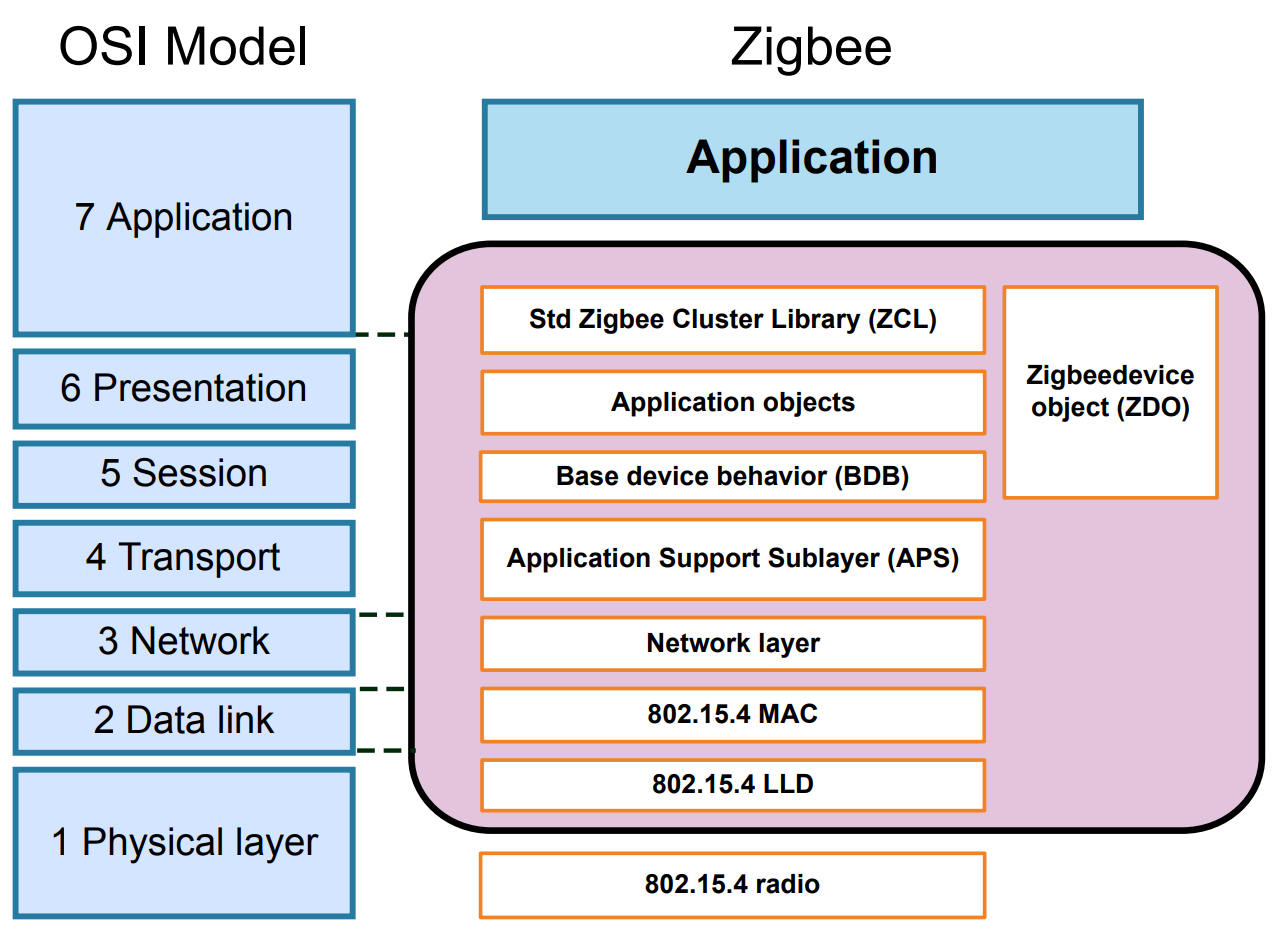
\includegraphics[width=0.618\linewidth]{zigbee_osi_comparison_an5506.png}
	\caption{Zestawienie warstw stosu ZigBee z modelem referencyjnym OSI. Źródło:~\cite{stmicroelectronics_an5506_2020}}
	\label{rys:zigbee_osi_comparison_an5506}
\end{figure}

ZigBee wprowadza termin \textit{profili}, będący kontraktem pomiędzy komunikatami wysyłanymi pomiędzy urządzeniami. Definiuje on
logiczną strukturę danych i zapewniając kompatybilność pomiędzy platformami różnych producentów. Cechą tą charakteryzują
się przede wszystkim profile publiczne zdefiniowane przez ZigBee Alliance. Poszczególni producenci mogą 
również opracować własnościowe, zamknięte struktury do tworzenia wewnętrznych sieci, gdzie kompatybilność pomiędzy
urządzeniami wielu producentów nie jest wymagana~\cite{zigbee_alliance_zigbee_2017, stmicroelectronics_an5506_2020, zigbee_alliance_zigbee_2017}.

\section{OpenThread}
\lipsum[1-10]

\section{Bluetooth Low Energy}
\lipsum[1-10]

\section{Porównanie przedstawionych standardów} % jako podroździał
% historia jako delikatny wstęp
\url{https://www.silabs.com/documents/public/application-notes/an1142-mesh-network-performance-comparison.pdf}
\url{https://www.silabs.com/wireless/matter}
\lipsum[1-15]


% 1. Krótki rys historyczny standardu
% 2. Opis stosu + jakiś obrazek
% 2.1. Częstotliwości na których pracuej standard
% 3. Topologia, rodzaje węzłów
